\section{Motivation}

Unmanned aerial vehicles (UAVs), commonly known as a drones, are replacing human pilots in potentially dangerous military missions. They are frequently deployed in missions of destroying enemy forces in denied environments. \cite{westra_2009, kacena1995}. One of the most reported cases in the beginning of 2020, regarding UAV's missions in military context, was the death o Iranian General Qasem Soleimani by an American UAV \cite{sarker_2020}. Another well known case was when the US special forces raided the safe-house of Osama Bin Laden in 2011 and caught him completely by surprise. In this mission, the UAVs were used to evade the Pakistani radar \cite{drew_2011}.

Due to the benefits of exploiting the surprise factor of monitored environments with aerial platforms, the use of stealth approaches becomes essential for mission success, because it allows missions to be conducted in proximity of threat radars and enemy air defences, by minimizing the signature of the aircraft, i.e., the traces left by the aircraft that can be used to detect it. According to Kacena \cite{kacena1995} stealth can be defined as a combination of techniques and technologies that aims at increasing the enemy's difficulty in detecting, tracking, guiding or predicting an object's future positions in space.

Regarding security, the use of manned airplanes for some missions may be risky, as it may endanger the life of the pilots \cite{venancio_2007}. On the other hand, UAVs can be sent into hostile areas with no risk to the lives of pilots \cite{mod_2011, foust_2012}. There are two classes of UAVs: non-autonomous and autonomous. For missions adopting non-autonomous UAVs, i.e., vehicles remotely controlled by a human operator, the mission success is directly related to the operator skills and to the endurance of the operator. Autonomous UAVs can perform actions such as detection, identification, targeting and engagement of an enemy faster than their non-autonomous counterparts \cite{bellamy_2015}.

Besides attack missions, UAVs can also be provide supply, maintenance, health services, and other services required by the soldiers of combat units to continue their missions in combat. According to \citeauthor{aeronautica_2012}, this kind of application is named Combat Service Support \cite{aeronautica_2012}. They can be used to deliver of combat supplies from a physical base or a vehicle to personnel engaged in combat operations or even reconnaissance missions. Examples of applications can include military equipment or even ambulance UAVs that deliver medicines, immunizations, and blood samples \cite{amukele_2017}. 

This kind of application is strong related with Vehicle Routing Problems (VRPs), because it is necessary to trace the route of each UAV. Also, depending on the  route, the whole mission can be compromised. According to \cite{toth_2002}, VRPs are characterized by the determination of the optimal set of routes to be performed by a fleet of vehicles to serve a given set of customers, and it is one of the most important, and studied, combinatorial optimization problems. According to \cite{thornton_2018}, current modes of drone-routing in military operations primarily involve the use of crewed supply vehicles and air drops, however the use of autonomous UAVs can provide several benefits.

In many applications, not all information about the problem instance is known prior. Considering delivery application, the most common dynamic events are the arrival of new customer requests. On the other hand, in military missions, it is necessary to consider that enemies can be discovered during the mission. Then, when a threat is detected, the UAVs need to react to the enemy in order to increase the probability of mission succeed  \cite{zhou_2018}. Also, the adjustment of the planned solution according to the plan in execution is another crucial factor and can be performed with different updating strategies. The class of vehicle-routing problem that modelling dynamic scenarios is named Dynamic Vehicle-Routing Problems (DVRP), also referred to as real-time or online VRP \cite{ritzinger_2016}. 

The Dynamic Vehicle Routing problem performed by several autonomous UAVs, considering an hostile environment, monitored by radars has not deeply studied in literature. We are assuming as the dynamic factor the unknown presence of enemy (enemy radars). The problem consists in visiting several waypoints and then return to the base, while minimizing the total flight time. Also, we will consider a time window, since UAVs have limited battery. The UAVs do not know about the presence of threats prior. Thus, as long as they detect a threat, they need to react in order to evade it, while perform stealth policies to reduce the exposure to the enemy. At this moment, the route need to be dynamically optimized, considering the presence of the enemy.  Figure \ref{fig:scenario} shows the proposed scenario. In this figure, the scenario is composed of 3 UAVs, 6 waypoints (represented by soldiers) an 3 threats. This scenario consider that 3 UAVs were not discovered yet by UAVs. However it is possible to see problem of static vehicle routing. The paths passes trough all the radars.

\begin{figure}[h!]
    \centering
    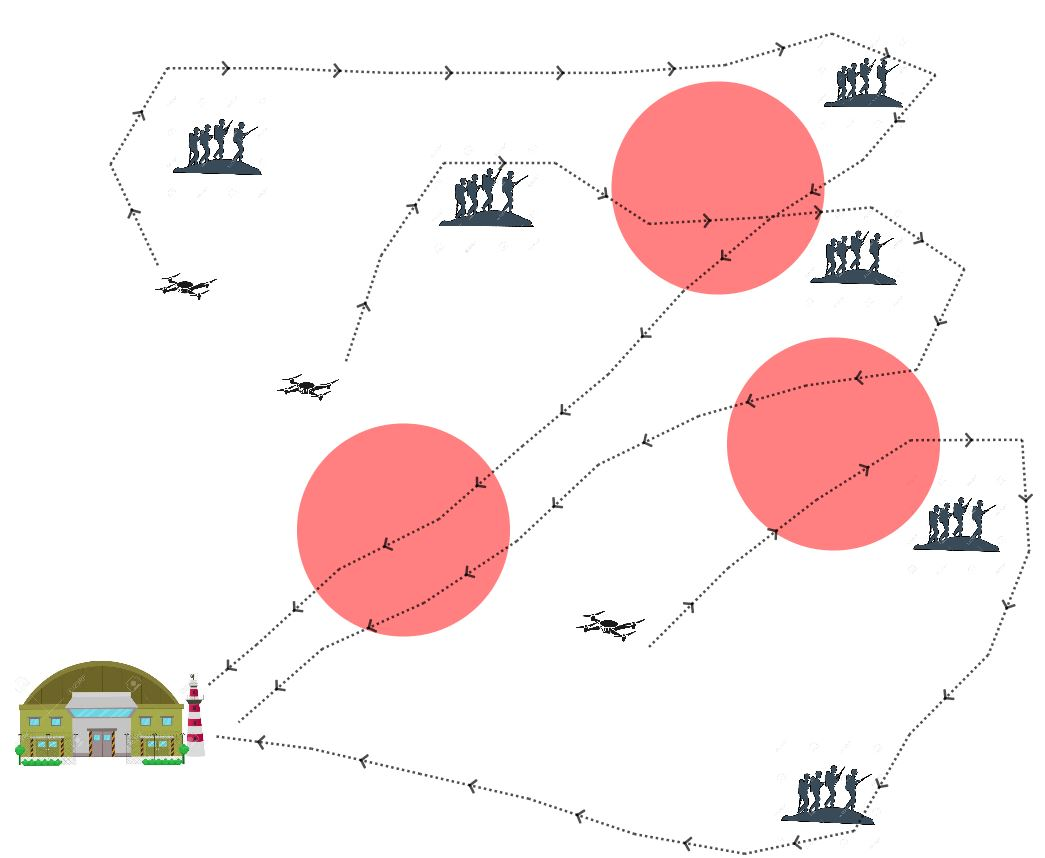
\includegraphics[width=0.6\textwidth]{Figures/scenario.JPG}
    \caption{An instance of the proposed scenario.}
    \label{fig:scenario}
\end{figure}


In this context, modelling a dynamic route optimization, considering multiple autonomous UAVs, assuming as the dynamic factor the unknown presence of enemy still is an open issue. The goal of this thesis is to propose a model that increases the UAVs stealthiness dynamically. This kind of problem can be considered as a DVRP. However, traditional DVRPs do not consider military operations and the impact of the stealthiness to the mission success.

\section{Objectives}

The goal of this thesis is to propose a model that increases stealth of autonomous UAVs during multi-target visiting missions. More specifically, it defines a model to reduce UAVs' exposure to threats through a combination of threat detection, path planning and dynamic route planning mechanisms.

We aim to assess the impact of different levels of hostility, regardless of UAVs stealth. Besides the reduction of flight time, the UAVs will try to increase their reliability, by adopting policies to detect and avoid threats. The evaluation of the model will consider three aspects: total flight time, stealth level of UAVs and the fraction of UAVs hit by the enemy.

\section{Contributions}

In this work we make the following contributions:

\begin{itemize}

    \item A review of logistical support missions in military environment. The result will be the identifications of  concepts, applications and peculiarities of logistics support missions to design simulation scenarios which correctly model their behavior.
    
    \item A review of state of art in DVRP. The result will be the study of models, that consider single and multiple UAVs, for the goods delivery. Moreover, we can select and evaluate appropriate models to be implemented in our scenario.
    
    \item We demonstrate how the coordinated use of multiple autonomous UAVs to perform routing affects the overall delivery time for logistical support missions, as well as the reliability of the delivery process. Our approach performs a route optimization while taking into account payload capacity and battery life.
    
    \item We demonstrate how the coordinate use of multiple UAVs can benefit logistical support in military operations. Our approach performs a Dynamic Route Optimization to re-plan the trajectory of UAVs when threats are discovered. Thi while trying to minimize the total flight time.
    
\end{itemize}


\section{Outline}
%The remaining of this work is organized as follows. In Chapter \ref{chap:2} we present the background of the research, addressing the way that military missions are performed and the importance of UAVs for missions and some of their characteristics. In addition, the stealth concept is described, relating its application to military missions performed by UAVs.

%In chapter \ref{chap:3} we present the related work of this research, emphasizing the characteristics of the stealth approach used in this work.

%Chapter \ref{chap:4} presents the computational model for improving stealthiness in collaborative UAV networks. The mechanism for detecting the threats and the stealth policy of UAVs to reduce the exposure to threats is detailed, as well as the way the UAVs move through the combination of control laws for path planning, coverage area improvement, connectivity robustness and maintenance.

%In chapter \ref{chap:5} we present the performed experiments to show the feasibility of our model, and a discussion about the achieved results for varying number of UAVs in the network and hostility level of the scenarios.

%Finally, Chapter \ref{chap:6} presents the conclusions, final considerations and proposals for extensions.


